\documentclass[12]{amsart}

\usepackage{amssymb,amsmath}

%\usepackage{refcheck}

\usepackage{graphicx}
\usepackage{amssymb}
\usepackage{mathrsfs}
\usepackage{amsmath}
\usepackage{latexsym}
\usepackage{amssymb}
\usepackage{enumerate}
\usepackage{fullpage} 
\usepackage{setspace}
\usepackage{color}
%\usepackage{ dsfont }
\usepackage{float}
\usepackage{physics}

%new math symbols taking no arguments
\newcommand\0{\mathbf{0}}
\newcommand\CC{\mathbb{C}}
\newcommand\FF{\mathbb{F}}
\newcommand\NN{\mathbb{N}}
\newcommand\QQ{\mathbb{Q}}
\newcommand\RR{\mathbb{R}}
\newcommand\ZZ{\mathbb{Z}}
\newcommand\bb{\mathbf{b}}
\newcommand\kk{\Bbbk}
\newcommand\mm{\mathfrak{m}}
\newcommand\pp{\mathfrak{p}}
\newcommand\xx{\mathbf{x}}
\newcommand\yy{\mathbf{y}}
\newcommand\GL{\mathit{GL}}
\newcommand\into{\hookrightarrow}
\newcommand\nsub{\trianglelefteq}
\newcommand\onto{\twoheadrightarrow}
\newcommand\minus{\smallsetminus}
\newcommand\goesto{\rightsquigarrow}
\newcommand\nsubneq{\vartriangleleft}

%redefined math symbols taking no arguments
\newcommand\<{\langle}
\renewcommand\>{\rangle}
\renewcommand\iff{\Leftrightarrow}
\renewcommand\phi{\varphi}
\renewcommand\implies{\Rightarrow}

%new math symbols taking arguments
\newcommand\ol[1]{{\overline{#1}}}

%redefined math symbols taking arguments
\renewcommand\mod[1]{\ (\mathrm{mod}\ #1)}

%roman font math operators
\DeclareMathOperator\aut{Aut}

%for easy 2 x 2 matrices
\newcommand\twobytwo[1]{\left[\begin{array}{@{}cc@{}}#1\end{array}\right]}

%for easy column vectors of size 2
\newcommand\tworow[1]{\left[\begin{array}{@{}c@{}}#1\end{array}\right]}

\newtheorem{theorem}{Theorem}[section]
\newtheorem{corollary}{Corollary}[theorem]
\newtheorem{lemma}[theorem]{Lemma}
\newtheorem{exercise}[theorem]{Exercise}

\title{Bosonic Codes for Pedestrians}
\author{Faris Sbahi}

\begin{document}
\maketitle

Quantum error correction is necessary to achieve fault tolerant quantum communication. In other words, one must implement a scheme to encode information redundantly into physical degrees of freedom so that information can be preserved in the presence of noise. One such scheme is continuous variable quantum information processing using bosonic modes\cite{braunstein1998error, braunstein2005quantum, niset2008experimentally, aoki2009quantum, lloyd1998analog, lassen2010quantum}. In this case, one encodes information in the space corresponding to the occupation number of a harmonic oscillator. Hence, one can express the code subspace in terms of number states $\{\ket{n}\}^\infty_{n=0}$\cite{michael2016new}, position and momentum eigenstates $\{\ket{x}\}_{x\in\RR}$ and $\{\ket{p}\}_{p\in\RR}$ \cite{gottesman2001encoding}, or a few coherent states $\{\ket{\alpha}\}_{\alpha\in S}$ (for some finite set $S$)\cite{cochrane1999macroscopically}.

The first studied continuous variable scheme utilizing bosonic modes is known as the two-mode “dual-rail” encoding published in 1995 \cite{chuang1995simple}. Nowadays, there are several bosonic codes being evaluated in the fault tolerant quantum computation race. In this review, we'll consider a few of the most popular contenders: first, we'll study three popular single mode codes with impressive protection capabilities. Then, we'll consider the work of \cite{albert2017performance} to evaluate the performance of these codes. Finally, we'll consider hardware-efficient multi-mode extensions which are notable for their progress toward physical realizability.

\section{Introduction}

\subsection{Definitions}

The generic task of quantum error correction is to find two logical code words---a qubit---embedded in a large Hilbert space. The code words are required to be robust such that if any one of the single, independent errors $E_{l,k} \in \mathcal{E}$ occurs, no quantum information is lost and any quantum superposition of the logical code words can be faithfully recovered. This is equivalent to finding two logical code words $\ket{W_\sigma}$, where $\sigma = \uparrow, \downarrow$, that satisfy the quantum error correction criteria, known also as the Knill-Laflamme conditions\cite{nielsen2002quantum}.

\begin{align}
\label{eq:k-l}
\bra{W_\sigma} E_l^\dag E_k \ket{W_\sigma} = \alpha_{l, k} \delta_{\sigma, \sigma'}	
\end{align}

for all $E_{l,k} \in \mathcal{E}$ such that $\alpha_{l,k}$ are entries of a Hermitian matrix and independent of the logical words. The independence of entries $\alpha_{l,k}$ from the logical code words and the structure of the non-diagonal entries guarantee that the different errors are distinguishable and correctable.

Notationally, we'll refer to a harmonic oscillator's non-Hermitian creation and annihilation operators as $a^\dag$ and $a$, respectively. Furthermore, we define $n := a^{\dag }a$. Recall the relations, with respect to Fock states $\ket{n}$,

\begin{align*}
a^{\dagger }|n\rangle &={\sqrt {n+1}}|n+1\rangle, \qquad a|n\rangle={\sqrt {n}}|n-1\rangle \\
n\ket{n} &= n\ket{n} \\
[a,a^{\dag }]&=1, \qquad[n,a^{\dag }]=a^{\dag }, \qquad[n,a]=-a,
\end{align*}

Also, recall the definition of coherent states $\ket{\alpha}$ which refer to eigenstates of the annihilation operator,

$$
|\alpha\rangle =e^{-{|\alpha|^2\over2}}\sum_{n=0}^{\infty}{\alpha^n\over\sqrt{n!}}|n\rangle =e^{-{|\alpha|^2\over2}}e^{\alpha\hat a^\dagger}|0\rangle ~,
$$

We will call errors generated by action of $a$ "loss" errors, by $a^\dag$ "gain" errors, and by $n$ "dephasing" errors. 

\section{Bosonic Error Models}

It's especially important to consider a practical bosonic error model before designing a bosonic code because of the unique nature of photonic errors. In particular, photons are prone to loss, and photon-photon interactions are extremely weak. Hence, bosonic QEC codes focus on correcting photon-loss errors using very limited forms of photon-photon interactions while striving to be hardware efficient\cite{niu2018hardware}. 

We can describe this using the pure-loss channel, which is a model for broadband-line and free-space communication [3] and it is the most common incoherent error pro- cess in optical and microwave cavities [23]. The second most common error is cavity dephasing, which is caused by fluctuations in the cavity frequency. Optical cavities have to be actively stabilized to fix the frequency, but the effects of such fluctuations are small relative to effects of energy loss, particularly in microwave cavities. There are also other coherent error processes, such as a Kerr non- linearity [29], which we briefly consider in Sec. VIII A.

The bosonic pure-loss channel is given by $N_\gamma = \exp(\kappa t D)$ ($\gamma$ defined below) with superoperator $D(\cdot) = a a^\dag - 1/2 \{ n , \cdot \}$ with $\kappa$ as the excitation loss rate and time interval $t$\cite{albert2017performance}. Another way to represent this is in the Kraus representation with Kraus operators

$$
E_l = \Big(\frac{\gamma}{1-\gamma}\Big)^{l / 2} \frac{a^l}{\sqrt{l!}}(1 - \gamma)^{n / 2}
$$

where $\gamma = 1 - \exp(- \kappa t)$. This is derived by integrating over all the possible jump times of exactly $l$ photon jumps during the time interval $\kappa t$\cite{chuang1997bosonic}. Therefore, the channel can be described as 

$$
N_\gamma = \sum_l^\infty E_l \rho E_l^\dag
$$

for density operator $\rho$.

Observe that this channel does not contain identity as a Kraus operator for $\gamma \neq 0$ due to damping/back-action $(1-\gamma)^{n / 2}$. So, even if there is no loss, there is still redistribution of probabilities of being in Fock states. Furthermore, this redistribution takes place over continuous time. 

\section{Single Mode Codes}

First, we emphasize why we must establish new codes for bosonic systems, in the first place. What if we used a simple encoding of $M$ qubits: $2^M$ Fock states cover photon numbers $0, 1, . . . , (2^{M - 1})$. Use binary representation: $\ket{n} = \ket{b_{M-1} b_{M-2} \cdots b_0 }$. The $j$th binary digit represents the eigenvalue $(1 + Z_j)/2$ for the corresponding physical qubit. E.g., $n=8$: $\ket{1000}$. Photon loss occurs, $a : \ket{1000} \mapsto \ket{0111}$. Hence, as the authors of \cite{michael2016new} note, QEC schemes based on models of independent single qubit errors cannot be easily transferred to this problem. Luckily, the stabilizer formalism provides useful intuition for codes we'll discuss

\subsection{A Simple Example}

So, consider a simple bosonic code to protect against $\mathcal{E} = \{ I, a \}$. Define $\ket{W_\uparrow} = \frac{\ket{0} + \ket{4}}{2}$, $\ket{W_\downarrow} = \ket{2}$. Hence, $\ket{E_1} = \ket{3}$ and $\ket{E_2} = \ket{1}$. We can distinguish states by measuring number and checking mod 4. Observe that both logical states have the same mean photon number i.e. $\bra{W_\sigma} n \ket{W_\sigma} = 2$. Therefore, $a : \alpha\ket{W_\uparrow} + \beta\ket{W_\downarrow} \mapsto \alpha \ket{E_1} + \beta \ket{E_2}$ (no deformation).

How can we generalize from here? Well, we can add greater spacing between states so that we can detect higher order loss errors or alternatively gain errors. Furthermore, observe that action by $n$ "dephases" (see how it can shift relative phases?). This leads to a superposition of codewords and error words. Project onto word basis to recover (efficient).

\subsection{Cat Codes}

Cat codes were first discovered in \cite{cochrane1999macroscopically} in the case of a single mode. Several papers have extended these codes to the multi-mode case in order to correct more errors or offer a hardware-efficient implementation\cite{albert2018multimode, leghtas2013hardware, mirrahimi2014dynamically} and we will summarize these results in Section \ref{sec:multi-cat}.

Now, consider using a superposition of "well-separated" coherent states as the logical state encoding. For example, consider a simple case

\begin{align*}
\ket{C^\alpha_{\uparrow/\downarrow}} &= N_{\uparrow /\downarrow} (\ket{\alpha} \pm \ket{i \alpha} + \ket{-\alpha} \pm \ket{-i \alpha}) \\
&= N_{\uparrow /\downarrow} \sum_{p\text{ even/odd}}^{[0, \infty)}\sqrt{\exp(-|\alpha|^2)\frac{
\alpha^{4p}}{2p!}}\ket{2p}
\end{align*}

where $N_{\uparrow /\downarrow}$ are the normalization factors which evidently become equal as $\alpha \rightarrow \infty$. Similarly, as $\alpha \rightarrow \infty$, $\bra{C^\alpha_{\uparrow}} N^p \ket{C^\alpha_{\uparrow}} = \bra{C^\alpha_{\downarrow}} N^p \ket{C^\alpha_{\downarrow}}$ which implies that cat states are potentially immune from any order of dephasing.

- explain why normalization factors approximate error correction unmet

Remember: distributed as Poisson and for large $N$, Binomial and Poisson approach normal distribution

Loss takes coherent states to coherent states! Can measure mod $S+1$ again to determine whether jump occurred. Do we do anything, if not


two different coherent states are not orthogonal,

$$
{\displaystyle \langle \beta |\alpha \rangle =e^{-{1 \over 2}(|\beta |^{2}+|\alpha |^{2}-2\beta ^{*}\alpha )}\neq \delta (\alpha -\beta )} \langle\beta|\alpha\rangle=e^{-{1\over2}(|\beta|^2+|\alpha|^2-2\beta^*\alpha)}\neq\delta(\alpha-\beta)
$$

(linked to the fact that they are eigenvectors of the non-self-adjoint annihilation operator â).

$$
|\alpha\rangle =e^{-{|\alpha|^2\over2}}\sum_{n=0}^{\infty}{\alpha^n\over\sqrt{n!}}|n\rangle =e^{-{|\alpha|^2\over2}}e^{\alpha\hat a^\dagger}|0\rangle ~,
$$

The notation ${\displaystyle |\alpha \rangle }$  does not refer to a Fock state. For example, when $\alpha = 1$, one should not mistake ${\displaystyle |1\rangle }$ for the single-photon Fock state, which is also denoted ${\displaystyle |1\rangle } $  in its own notation. 

The expression ${\displaystyle |\alpha \rangle } $  with $\alpha = 1$ represents a Poisson distribution of number states ${\displaystyle |n\rangle }$  with a mean photon number of unity.

\subsection{Binomial Codes}

\begin{itemize}
\item Protect against $\mathcal{E} = \{I, a, a^2, \cdots, a^L, a^\dag, \cdots, (a^\dag)^G, N, \cdots, N^D \}$
\item Consider

$$
\ket{W_{\uparrow / \downarrow}} = \frac{1}{\sqrt{2^N}} \sum_{ p\text{ even/odd}}^{[0, N+1]} \sqrt{\binom{N+1}{ p }} \ket{p(S+1)}
$$

with $S = L+G$, $N = \max\{L, G, 2D\}$.

\item Now, trust me that it works similarly to before!
\item Mean photon numbers equal (no deformation) and QEC condition holds
\item Can be shown by writing difference in $l$th moment of photon number of codewords as $l$th derivative of $(1+x)^{N+1}\vert_{x=-1}$ with $l \leq \max\{L, G\}$ up to a factor
\item Measure photon number mod $S+1$
\end{itemize}

The Fock state distributions of the binomial and cat codes are binomial and Poissonian, respectively. As the average number of photons is increased (larger N), both of these distributions approach a normal distribution, and so the binomial and cat codes asymptotically approach each other. 

\begin{figure}[H]
\centering
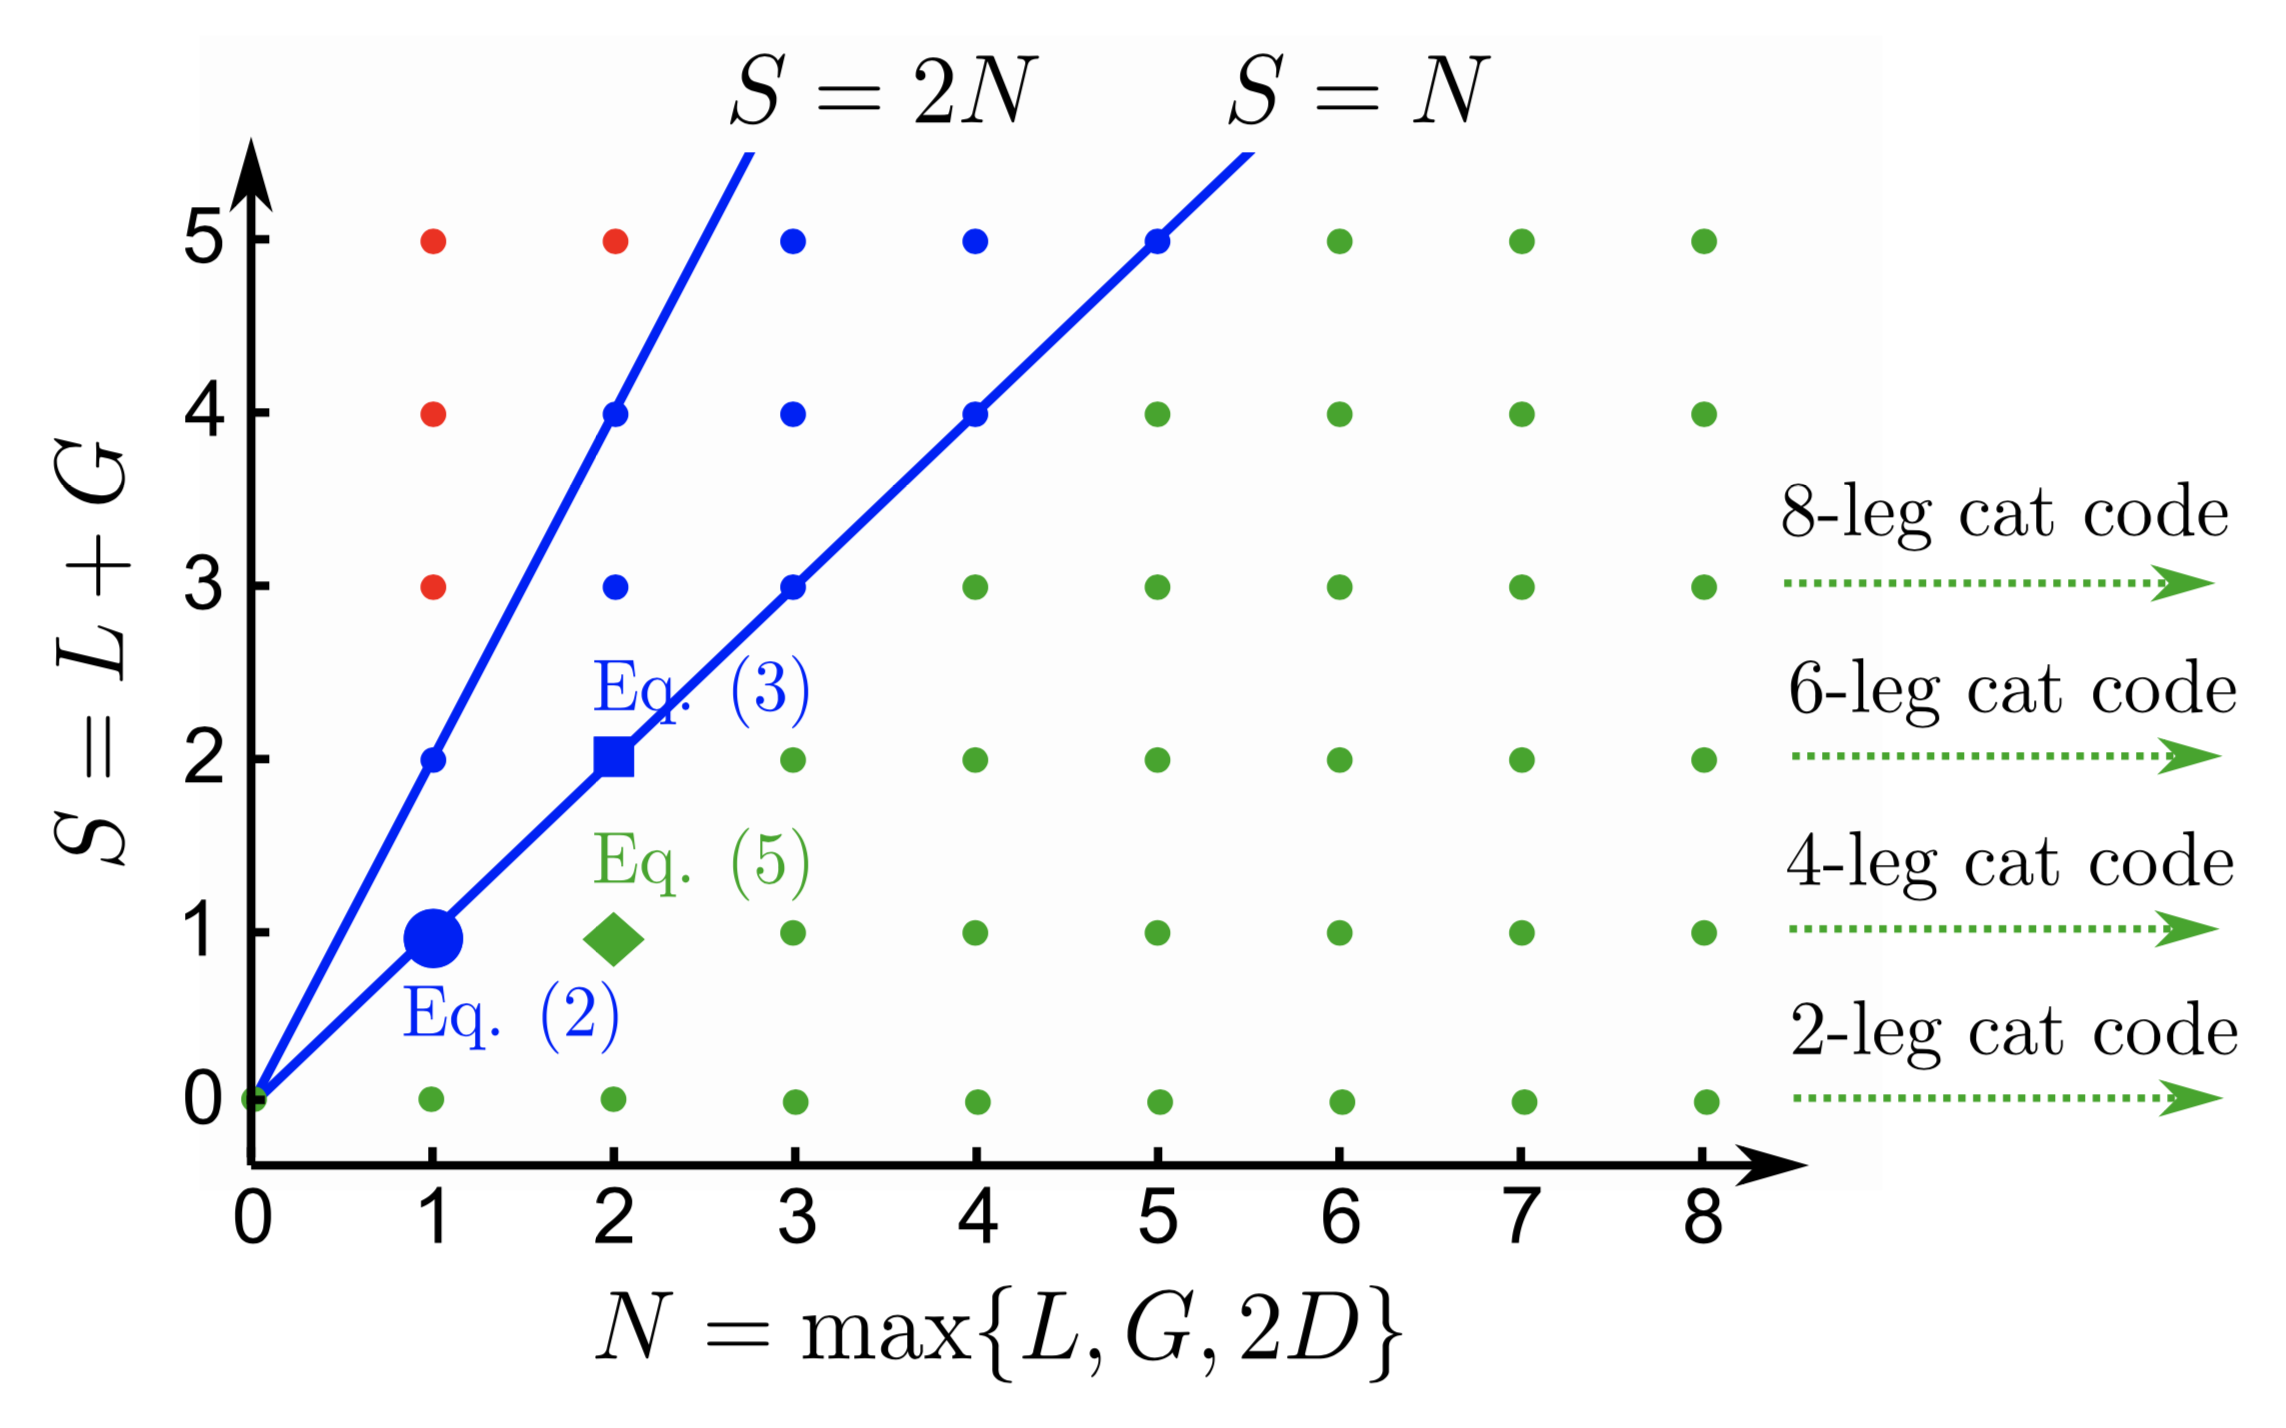
\includegraphics[width=0.5\linewidth,keepaspectratio]{binom_cat.png}	
\caption{Figure borrowed from \cite{michael2016new} comparing binomial codes to cat codes. Observe that, in principle, unlimited dephasing errors can be tolerated by cat codes.}
\end{figure}

\subsection{GKP Codes}

\begin{itemize}
\item Use the continuous basis of non-normalizable eigenstates of the position operator $x$	
\item Not enough time!
\item Quantum analoge of frequency combs
\item Key: protect against displacement errors $D_\alpha = \exp{\alpha a^\dag  - \alpha* a}$, not loss errors explicitly
\end{itemize}

\section{Discussion}

\subsection{Performance Comparisons}

VV Albert considers "channel fidelity", $F_\mathcal{E}$, which is the overlap between the initial state and the final state when considering an initial Bell state such that only the first qubit is acted on by the channel

Optimal recovery for each code is computable via a semi-definite program

\begin{figure}[H]
\centering
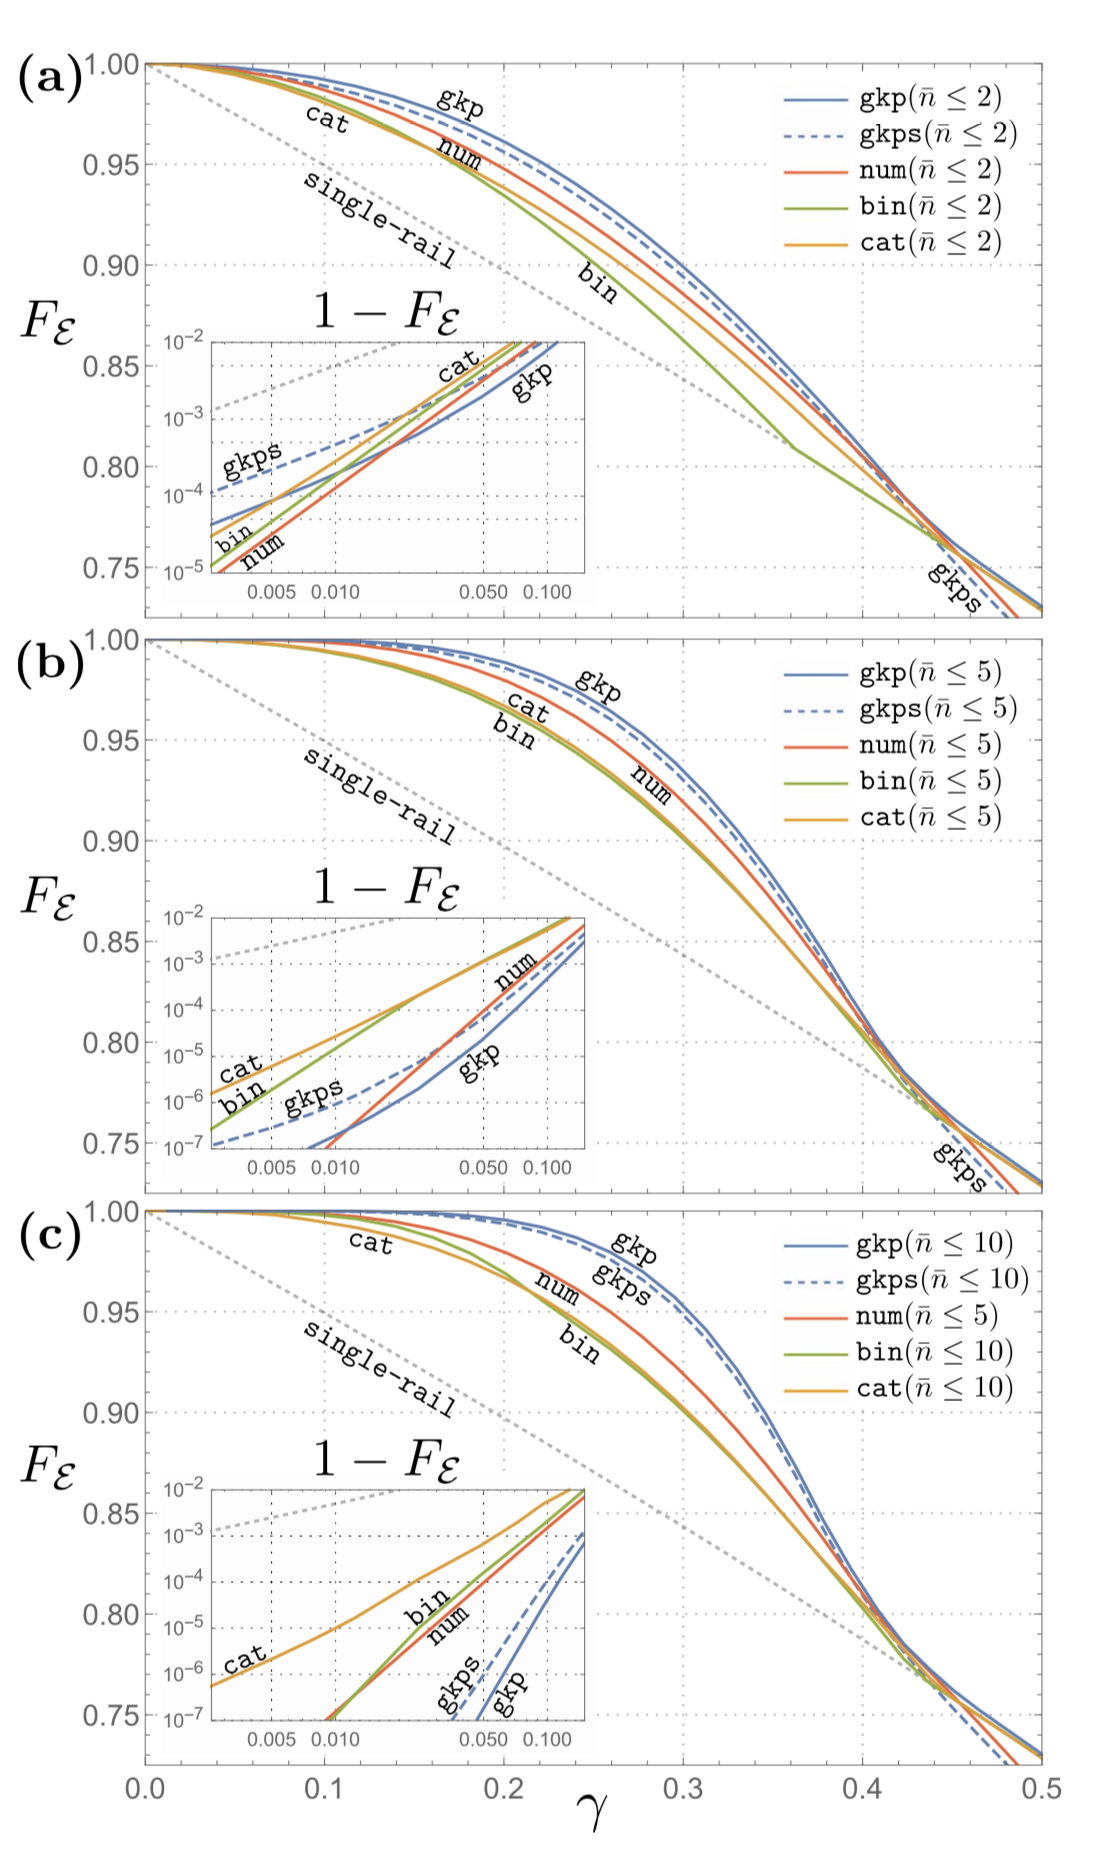
\includegraphics[width=0.5\linewidth,keepaspectratio]{fidelity.png}	
\end{figure}

\subsection{Multi-Mode Extensions}

\subsubsection{Cat Codes}\label{sec:multi-cat}

\begin{itemize}
		\item Pair-cat codes (VV Albert)
		\item Reduction in order of nonlinearity required for physical realization (as with $\chi(2)$)
		\item With ordinary cat codes and current technology, the number parity syndrome makes it difficult to realize simultaneous discrete (usually for loss) and continuous error correction  (usually for dephasing)
	\end{itemize}
	
\subsubsection{Binomial Codes}

Hardware Efficient Constructions

Noon codes

\begin{itemize}
	\item To create more useful quantum superpositions of Fock states which can store quantum information, it is necessary to couple the bosonic mode to a non-linear element, e.g., a superconducting qubit, a trapped ion, or a Rydberg atom
		\item $\chi(2)$ code uses $O(n)$ instead of $O(n^2)$ qubits that previous two mode codes had used to correct $m$ loss/gain/dephasing errors (Niu)
		\item Inspired by cat code, but uses lower order non-linearity
	\end{itemize}

\subsection{Broader Context}

\subsubsection{Continuous Variable Systems}

\subsubsection{Future Developments}

\nocite{*}
\bibliography{qec_final_project.bib}
\bibliographystyle{amsplain}

\end{document}


\section{Multi-Mode Extensions}

$a$ "loss 